\chapter{波函數、密度矩陣與定域性}

\lectureoverview{貝爾定理之所以延後討論，有一個關鍵原因：在追問貝爾定理禁止什麼之前，我們必須先精確說明糾纏的意義。若一個雙體態無法分解為 Alice 的一個態與 Bob 的一個態，它便是糾纏態。波函式讓這項判據具體呈現，關聯揭示其後果，而單重態則提供了決定性的例子。接著，約化密度矩陣成為糾纏整體中其中一部分的完整局域描述。有了這套工具，測量便呈現為造成糾纏的交互作用；系統--觀察者的界線可以移動而不改變預測；糾纏與定域性之間表面上的張力也就能明確表述：遠方的選擇會改變條件關聯，但不會改變可用於傳訊的無條件統計。}

\section{糾纏究竟意味著什麼}

人們很容易直接進入貝爾定理。這個定理十分優美，但其意義無法與它所檢驗的結構分開。因此，更迫切的問題還不是量子力學是否違反貝爾不等式，而是糾纏態對複合系統究竟說明了什麼。

一種常見說法是，兩個糾纏系統\emph{共享一個態}。這種說法並沒有區分出任何差異。每個複合系統都有一個態，無論它是否糾纏。差別在於能否因式分解。若 \(A\) 和 \(B\) 的希爾伯特空間分別是 \(\mathcal H_A\) 和 \(\mathcal H_B\)，則這對系統的態屬於
\begin{equation}
\mathcal H_{AB}=\mathcal H_A\otimes\mathcal H_B.
\end{equation}
若一個純態可以寫成
\begin{equation}
\ket{\Psi}_{AB}=\ket{\psi}_A\otimes\ket{\phi}_B.
\label{eq:l7-product-state}
\end{equation}
它就是乘積態。若不存在這樣一對因子，\(\ket{\Psi}_{AB}\) 就是糾纏態。

\begin{classroomqa}
\audiencequestion{糾纏是否只表示兩個系統出現在同一個態向量中？}
\lecturerresponse{不是。乘積態也屬於整對系統的希爾伯特空間。糾纏是更強、且與基底無關的陳述：整體的向量無法寫成 Alice 的一個向量乘上 Bob 的一個向量。}
\end{classroomqa}

\begin{classroomqa}
\audiencequestion{巧妙地變換基底，能把糾纏態變成乘積態嗎？}
\lecturerresponse{若基底變換是局域的，也就是分別對 Alice 和 Bob 變換基底，就不能。局域基底變換會改變各因子的座標，但不會改變態能否因式分解。聯合希爾伯特空間中完全任意的基底或許會掩蓋張量積結構，卻不會改變哪些物理自由度屬於 Alice、哪些屬於 Bob。}
\end{classroomqa}

\section{波函數作為希爾伯特空間中的座標}

\emph{波函數}一詞帶有歷史意象，但這些意象並不屬於它的數學定義。波函數是態向量在選定基底中的座標表示。設一組完備的對易可觀測量具有共同本徵向量
\begin{equation}
\ket{a,b,c,\ldots}.
\end{equation}
這些標記必須完備：合起來能區分基底中的每一個向量。於是
\begin{align}
\ket{\Psi}
&=\sum_{a,b,c,\ldots}
\ket{a,b,c,\ldots}
\braket{a,b,c,\ldots}{\Psi} \\
&=\sum_{a,b,c,\ldots}
\psi(a,b,c,\ldots)\ket{a,b,c,\ldots},
\label{eq:l7-wavefunction-expansion}
\end{align}
其中
\begin{equation}
\psi(a,b,c,\ldots)
=\braket{a,b,c,\ldots}{\Psi}.
\label{eq:l7-wavefunction-definition}
\end{equation}
連續標記所對應的求和則改為積分。

\begin{figure}[htbp]
\centering
\includegraphics[width=0.88\textwidth]{lecture_07_figure_01.png}
\caption{波函數是態在完備基底中的係數集合。}
\lectureframe{00:07:00}
\end{figure}

對於三維空間中的粒子，對易標記可以是 \(x,y,z\)，而
\begin{equation}
\psi(x,y,z)=\braket{x,y,z}{\Psi}
\end{equation}
就是 Schr\"odinger 熟悉的位置空間波函數。對於 \(\sigma_z\) 基底中的單一自旋，波函數只有一對分量：
\begin{equation}
\psi(u)=\braket{u}{\Psi},
\qquad
\psi(d)=\braket{d}{\Psi}.
\end{equation}
兩個自旋則需要兩個標記：
\begin{equation}
\Psi(a,b)=\braket{a,b}{\Psi},
\qquad
a,b\in\{u,d\}.
\label{eq:l7-two-spin-wavefunction}
\end{equation}
這個定義並不要求空間中存在字面意義上的波。

\begin{classroomqa}
\audiencequestion{改變波函數的基底就是傅立葉變換嗎？}
\lecturerresponse{傅立葉變換是位置表象與動量表象之間的一種特定基底變換。更一般地說，任何正交歸一基底的變換，都是座標的么正變換。從 \(\sigma_z\) 基底轉到 \(\sigma_x\) 基底，類似於傅立葉變換；不過這裡是有限維的么正矩陣，而非位置--動量之間的積分變換。}
\end{classroomqa}

\begin{classroomqa}
\audiencequestion{如果波函數隨基底變換而改變，物理態也改變了嗎？}
\lecturerresponse{沒有。右矢 \(\ket{\Psi}\) 是抽象的態；數值 \(\psi(a,b,c,\ldots)\) 則是它在所選基底中的座標。改變座標會改變這些數值，但向量本身及所有物理預測都不變。}
\end{classroomqa}

\section{期望值的分量表示}

在引入密度矩陣之前，先展開期望值的分量結構。設 \(L\) 是一個可觀測量，其矩陣元為
\begin{equation}
L_{a'a}=\bra{a'}L\ket{a}.
\label{eq:l7-matrix-elements}
\end{equation}
若 \(\ket{\Psi}=\sum_a\psi(a)\ket{a}\)，則
\begin{align}
\expect{L}
&=\bra{\Psi}L\ket{\Psi} \\
&=\sum_{a',a}
\psi^*(a')\bra{a'}L\ket{a}\psi(a) \\
&=\sum_{a',a}\psi^*(a')L_{a'a}\psi(a).
\label{eq:l7-expectation-components}
\end{align}

\begin{figure}[htbp]
\centering
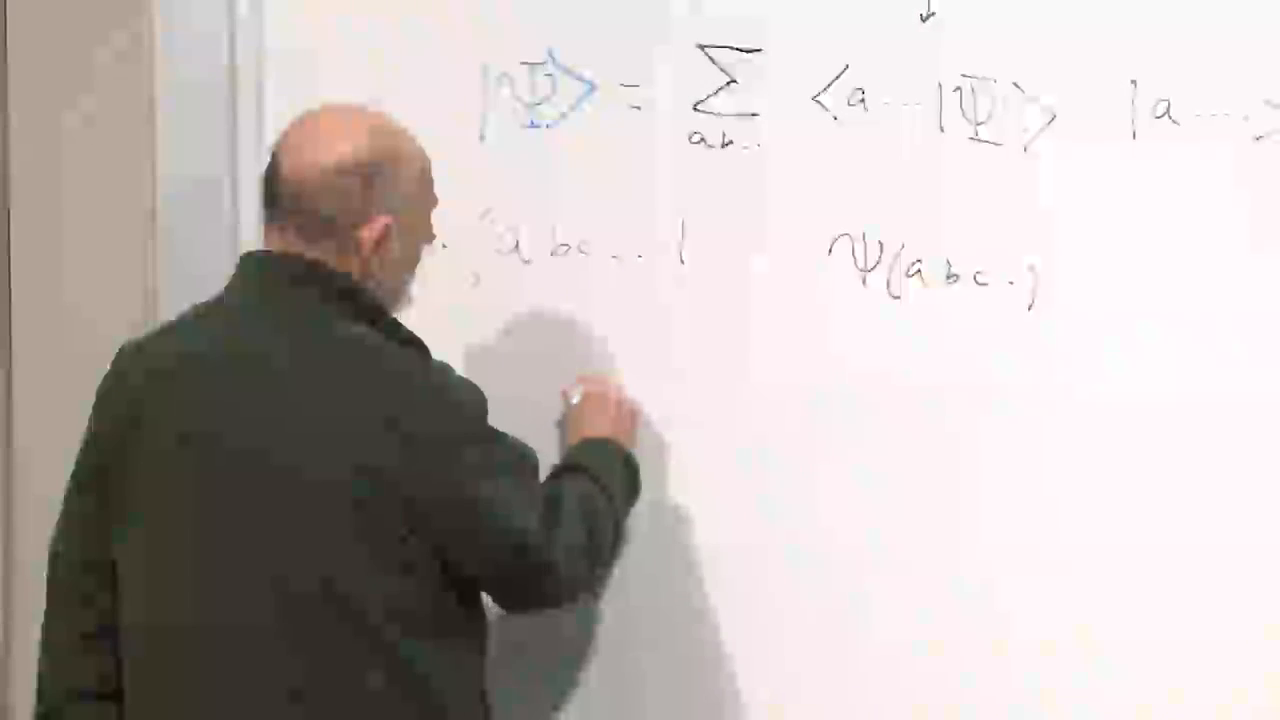
\includegraphics[width=0.88\textwidth]{lecture_07_figure_02.png}
\caption{將期望值的夾心式展開為波函數係數與矩陣元。}
\lectureframe{00:14:08}
\end{figure}

現在將系統分為 Alice 的部分和 Bob 的部分。設 \(a\) 是 Alice 的完備基底標記，\(b\) 是 Bob 的完備基底標記：
\begin{equation}
\ket{\Psi}_{AB}
=\sum_{a,b}\Psi(a,b)\ket{a,b}.
\label{eq:l7-composite-expansion}
\end{equation}
只屬於 Alice 的可觀測量，在複合空間中的表示為
\begin{equation}
L_A=L\otimes I_B,
\end{equation}
因此其矩陣元為
\begin{equation}
\bra{a',b'}L_A\ket{a,b}
=L_{a'a}\delta_{b'b}.
\label{eq:l7-alice-local-matrix}
\end{equation}
同理，局域於 Bob 的可觀測量具有形式
\begin{equation}
M_B=I_A\otimes M,
\qquad
\bra{a',b'}M_B\ket{a,b}
=\delta_{a'a}M_{b'b}.
\label{eq:l7-bob-local-matrix}
\end{equation}
未作用因子上的單位算符，正是 Alice 的操作作用於 Alice、Bob 的操作作用於 Bob 這項事實的數學表述。

將式~\eqref{eq:l7-alice-local-matrix}代入期望值，可得
\begin{equation}
\expect{L_A}
=\sum_{a',a,b}
\Psi^*(a',b)L_{a'a}\Psi(a,b).
\label{eq:l7-local-expectation}
\end{equation}
這個公式已包含約化密度矩陣；先看看因式分解的作用，之後再重新整理這個公式。

\begin{classroomqa}
\audiencequestion{為什麼式~\eqref{eq:l7-local-expectation}中 Bob 的指標只剩一個？}
\lecturerresponse{Bob 空間上的單位算符貢獻了 \(\delta_{b'b}\)。它會令 Bob 一側的 bra 與 ket 標記相等，因此對 \(b',b\) 的雙重求和便化為對 \(b\) 的單一求和。}
\end{classroomqa}

\begin{classroomqa}
\audiencequestion{Alice 需要知道 Bob 使用哪個基底嗎？}
\lecturerresponse{Bob 使用哪個基底都不會影響任何物理預測。對 Bob 的完備基底求和，就是單位算符的完備分解。換用不同的 Bob 基底會改變各個分量 \(\Psi(a,b)\)，卻不會改變 Alice 的期望值。}
\end{classroomqa}

\section{乘積態與關聯}

乘積態的聯合波函數可以因式分解：
\begin{equation}
\Psi(a,b)=\psi_A(a)\phi_B(b).
\label{eq:l7-wavefunction-factorization}
\end{equation}
將它代入式~\eqref{eq:l7-local-expectation}：
\begin{align}
\expect{L_A}
&=\sum_{a',a,b}
\psi_A^*(a')\phi_B^*(b)
L_{a'a}
\psi_A(a)\phi_B(b) \\
&=\left[
\sum_{a',a}\psi_A^*(a')L_{a'a}\psi_A(a)
\right]
\left[
\sum_b|\phi_B(b)|^2
\right] \\
&=\bra{\psi_A}L\ket{\psi_A}.
\label{eq:l7-product-local-expectation}
\end{align}
Bob 的歸一化使他的因子等於一。因此，Alice 的局域統計與完全沒有引入 Bob 系統時相同。

\begin{figure}[htbp]
\centering
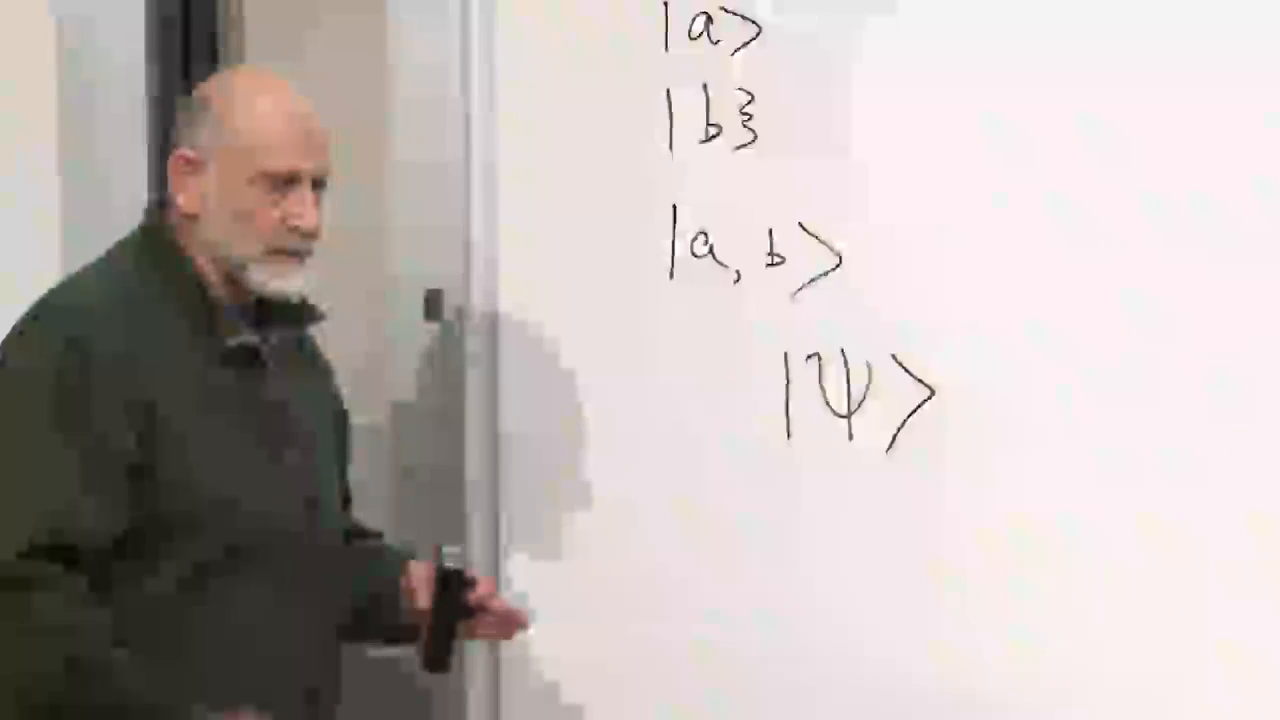
\includegraphics[width=0.88\textwidth]{lecture_07_figure_03.png}
\caption{聯合波函數的因式分解，以及相應的局域期望值分離。}
\lectureframe{00:29:18}
\end{figure}

Alice 的一個可觀測量與 Bob 的一個可觀測量相乘，其矩陣元為
\begin{equation}
\bra{a',b'}L_A M_B\ket{a,b}
=L_{a'a}M_{b'b}.
\end{equation}
對乘積態而言，期望值會分離：
\begin{equation}
\expect{L_A M_B}
=\expect{L_A}\expect{M_B}.
\label{eq:l7-product-correlation-factorization}
\end{equation}
因此，自然可以定義連通關聯
\begin{equation}
C(L,M)
=\expect{L_A M_B}
-\expect{L_A}\expect{M_B}.
\label{eq:l7-connected-correlation}
\end{equation}
對每一對局域可觀測量而言，所有乘積態都有 \(C(L,M)=0\)。反過來說，對純雙體態而言，糾纏保證至少有一對局域可觀測量具有非零連通關聯。

\begin{classroomqa}
\audiencequestion{\(L_A M_B\)是否表示先測量 Bob，再測量 Alice？}
\lecturerresponse{不是。算符作用於態向量，測量則由儀器執行。這個乘積表示先作用 \(M_B\)，再作用 \(L_A\)。由於兩個算符分別作用於不同的張量因子，\([L_A,M_B]=0\)，所以在數學上，作用次序並不重要。至於如何在實驗室中估計聯合期望值，則是另一回事。}
\end{classroomqa}

\begin{classroomqa}
\audiencequestion{即使某個選定的關聯為零，態仍可能是糾纏態嗎？}
\lecturerresponse{當然可能。某個 \(C(L,M)\) 為零，只表示這一對特定的可觀測量彼此不相關。要確認純態可以因式分解，所有局域交叉關聯都必須能因式分解。部分關聯也不一定能用某個簡單的單一數值表示部分糾纏；完整的約化密度矩陣譜才包含這項資訊。}
\end{classroomqa}

\begin{classroomqa}
\audiencequestion{所有具有關聯的態都是糾纏態嗎？}
\lecturerresponse{對於這裡討論的純態，無法因式分解的關聯揭示了糾纏。對混合態而言，一般的古典關聯也能使 \(C(L,M)\neq0\)。因此，稍後的密度矩陣判準必須加上條件：整體的態是否已知為純態。}
\end{classroomqa}

\section{單態：整體確定，部分不確定}

設 \(\boldsymbol{\sigma}\) 作用於 Bob 的自旋，\(\boldsymbol{\tau}\) 作用於 Alice 的自旋。兩者的單態為
\begin{equation}
\ket{S}
=\frac{1}{\sqrt2}
\left(\ket{u d}-\ket{d u}\right),
\label{eq:l7-singlet}
\end{equation}
第一個位置代表 Bob，第二個代表 Alice。兩個自旋的 \(z\) 分量都沒有確定值：
\begin{equation}
\expect{\sigma_z}=0,
\qquad
\expect{\tau_z}=0.
\label{eq:l7-singlet-local-z}
\end{equation}
然而，兩者的乘積有確定值：
\begin{equation}
\expect{\sigma_z\tau_z}=-1.
\label{eq:l7-singlet-product-z}
\end{equation}
每次測量 \(z\) 分量，結果都相反。

旋轉不變性使這項陳述不受方向影響。對任意單位向量 \(\mathbf n\)，
\begin{equation}
\expect{\boldsymbol{\sigma}\cdot\mathbf n}
=\expect{\boldsymbol{\tau}\cdot\mathbf n}=0,
\qquad
\expect{
(\boldsymbol{\sigma}\cdot\mathbf n)
(\boldsymbol{\tau}\cdot\mathbf n)
}=-1.
\label{eq:l7-singlet-any-axis}
\end{equation}
更一般地，
\begin{equation}
\expect{\sigma_i\tau_j}=-\delta_{ij}.
\label{eq:l7-singlet-correlation-tensor}
\end{equation}
每個部分都完全無極化，而沿相同軸測得的結果則完全反相關。

\begin{figure}[htbp]
\centering
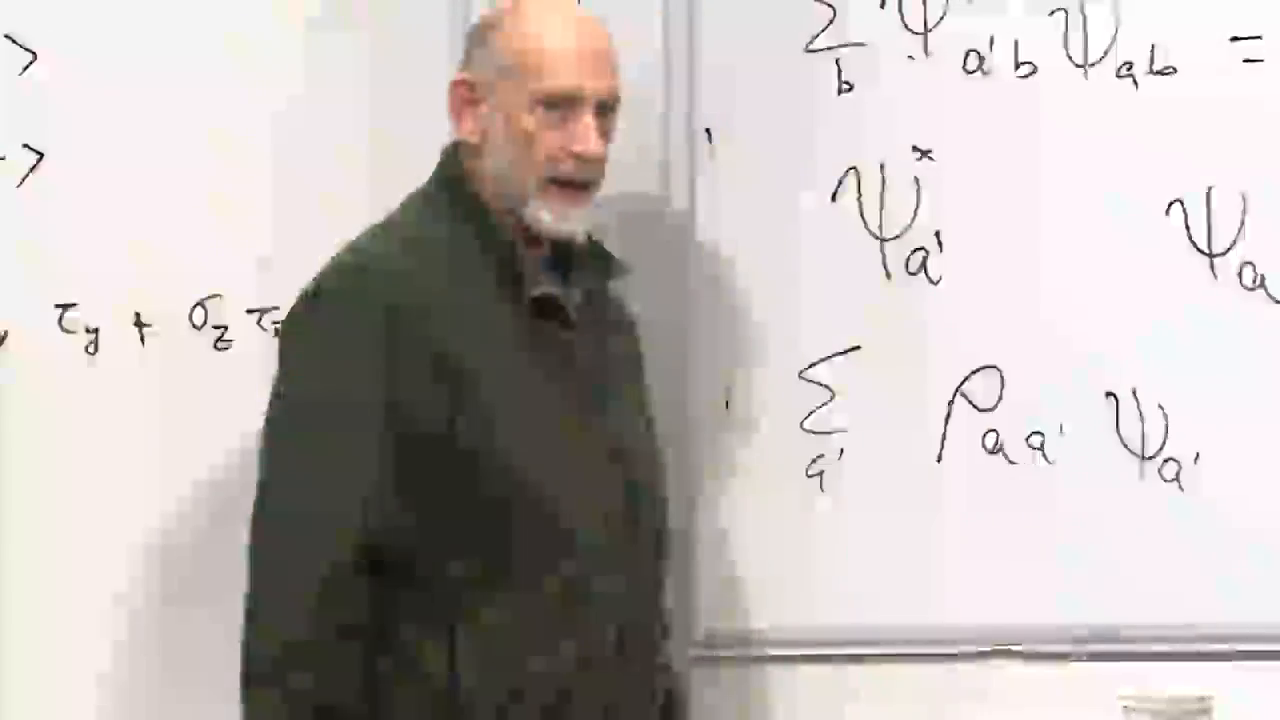
\includegraphics[width=0.88\textwidth]{lecture_07_figure_04.png}
\caption{對單態而言，每個局域自旋的平均值皆為零，而相同分量的乘積為 \(-1\)。}
\lectureframe{00:38:28}
\end{figure}

這是糾纏造成的典型反轉。孤立自旋若處於純態，總有某個方向上的自旋值是確定的。但在單態中，無論沿哪個方向，都無法使任一局域自旋的值確定。儘管如此，複合態仍是純態，而且已被完全指定。對整體的了解已達量子力學所允許的極限，我們卻仍無法為其中任何一部分指定純態。

\begin{classroomqa}
\audiencequestion{如果我們已精確知道整體的態，為什麼不能推知每個自旋都有確定的態？}
\lecturerresponse{因為單態不是乘積態。它的係數無法分解成 Bob 的振幅乘上 Alice 的振幅。資訊存在於兩部分之間的關係，而不是存在於兩個各自獨立的局域波函數中。}
\end{classroomqa}

\begin{classroomqa}
\audiencequestion{像 \(\sigma_z\) 這樣的算符本身可能是自旋的態嗎？}
\lecturerresponse{不是。態是向量，或更一般地說，是密度算符；\(\sigma_z\)則是作用於態上的可觀測量。\(\sigma_z\)的本徵向量是具有確定 \(z\) 分量的態，但可觀測量與其本徵向量是不同類型的物件。}
\end{classroomqa}

\begin{classroomqa}
\audiencequestion{寫下 \(\sigma_z\tau_z\ket{S}=-\ket{S}\) 時，我們是否已經進行測量？}
\lecturerresponse{沒有。這個方程描述算符如何作用於向量。它表示若測量相應的聯合可觀測量，結果必定是 \(-1\)；但光是寫下本徵值方程，並沒有納入任何探測器。}
\end{classroomqa}

\begin{classroomqa}
\audiencequestion{一對糾纏粒子也可能只有部分相關嗎？}
\lecturerresponse{可能。沿相同軸完全反相關，是單態的一項特殊性質。其他糾纏態的關聯可能較弱；即使是單態，當兩軸不同時，得到的也是 \(-\mathbf a\cdot\mathbf b\)，而非 \(-1\)。糾纏關乎的是無法因式分解，而不是每次選定測量的結果都完全相同或完全相反。}
\end{classroomqa}

\section{透過能量弛豫製備單態}

旋轉不變的雙自旋算符
\begin{equation}
\boldsymbol{\sigma}\cdot\boldsymbol{\tau}
=\sigma_x\tau_x+\sigma_y\tau_y+\sigma_z\tau_z
\label{eq:l7-spin-dot-spin}
\end{equation}
將四維態空間分成不同部分。作用於單態時，
\begin{equation}
(\boldsymbol{\sigma}\cdot\boldsymbol{\tau})\ket{S}
=-3\ket{S},
\label{eq:l7-singlet-dot-eigenvalue}
\end{equation}
而三個三重態各自的本徵值都是 \(+1\)。

\begin{figure}[htbp]
\centering
\includegraphics[width=0.88\textwidth]{lecture_07_figure_05.png}
\caption{旋轉不變的耦合 \(\boldsymbol{\sigma}\cdot\boldsymbol{\tau}\)，以及它在區分單態與三重態子空間時所扮演的角色。}
\lectureframe{00:52:33}
\end{figure}

假設相互作用哈密頓量包含
\begin{equation}
H_{\mathrm{int}}
=J\,\boldsymbol{\sigma}\cdot\boldsymbol{\tau}.
\label{eq:l7-exchange-hamiltonian}
\end{equation}
對於反鐵磁耦合 \(J>0\)，單態的能量比三重態低
\begin{equation}
\Delta E=4J.
\end{equation}
讓兩個自旋彼此靠近，使較高能量的成分透過放出光子、聲子或其他激發而衰變，這對自旋便會弛豫至單態。之後可以將兩個自旋分開，同時保持其聯合態，前提是分開的過程不會引入不可控制的自旋旋轉，也不會過於突然地關閉能隙。

原子系統中也會出現相同的能量原理。例如在正電子素中，電子與正電子的自旋耦合會使單態與三重態組態分裂。根據 \(E=mc^2\)，能量差也對應質量差，但光譜學通常以能量或頻率表示這項分裂。

\begin{classroomqa}
\audiencequestion{單態總是兩個相互作用自旋的基態嗎？}
\lecturerresponse{不是。在式~\eqref{eq:l7-exchange-hamiltonian}中，符號為 \(J>0\) 時，單態才是基態。若符號相反，則三重態的能量較低。製備方式取決於實際的相互作用及其能量排序，而不能只看是否存在兩個自旋。}
\end{classroomqa}

\begin{classroomqa}
\audiencequestion{能否分別測量三個分量，以測出 \(\boldsymbol{\sigma}\cdot\boldsymbol{\tau}\)？}
\lecturerresponse{不能在同一對粒子上同時進行三種局域自旋測量：\(\sigma_x,\sigma_y,\sigma_z\)彼此不相容，三個 \(\tau\) 分量也是如此。可以分別沿 \(x,y,z\) 測量三組子系綜，再重建其期望值；也可以用適當的聯合儀器直接測量單態--三重態可觀測量。}
\end{classroomqa}

\begin{classroomqa}
\audiencequestion{兩個自旋分開後，必須持續相互作用才能保持糾纏嗎？}
\lecturerresponse{不必。製備或改變態需要相互作用；但單態一旦製備完成，么正演化便能在沒有粒子間持續作用力的情況下維持其糾纏。局域磁場可能使兩個因子旋轉，但局域么正旋轉本身不會破壞糾纏。}
\end{classroomqa}

\section{約化密度矩陣}

回到 Alice 的局域期望值：
\begin{equation}
\expect{L_A}
=\sum_{a',a,b}
\Psi^*(a',b)L_{a'a}\Psi(a,b).
\end{equation}
將不屬於 \(L\) 的因子重新整理：
\begin{equation}
\expect{L_A}
=\sum_{a',a}
\left[
\sum_b\Psi(a,b)\Psi^*(a',b)
\right]L_{a'a}.
\label{eq:l7-regrouped-expectation}
\end{equation}
方括號中的表示式就是 Alice 的約化密度矩陣：
\begin{equation}
(\rho_A)_{aa'}
=\sum_b\Psi(a,b)\Psi^*(a',b).
\label{eq:l7-reduced-density-components}
\end{equation}
用不依賴基底的記號表示，
\begin{equation}
\rho_A
=\operatorname{Tr}_B\ket{\Psi}\bra{\Psi},
\label{eq:l7-partial-trace}
\end{equation}
Alice 的每個局域期望值都是
\begin{equation}
\expect{L_A}
=\operatorname{Tr}_A(\rho_A L).
\label{eq:l7-density-expectation}
\end{equation}

\begin{figure}[htbp]
\centering
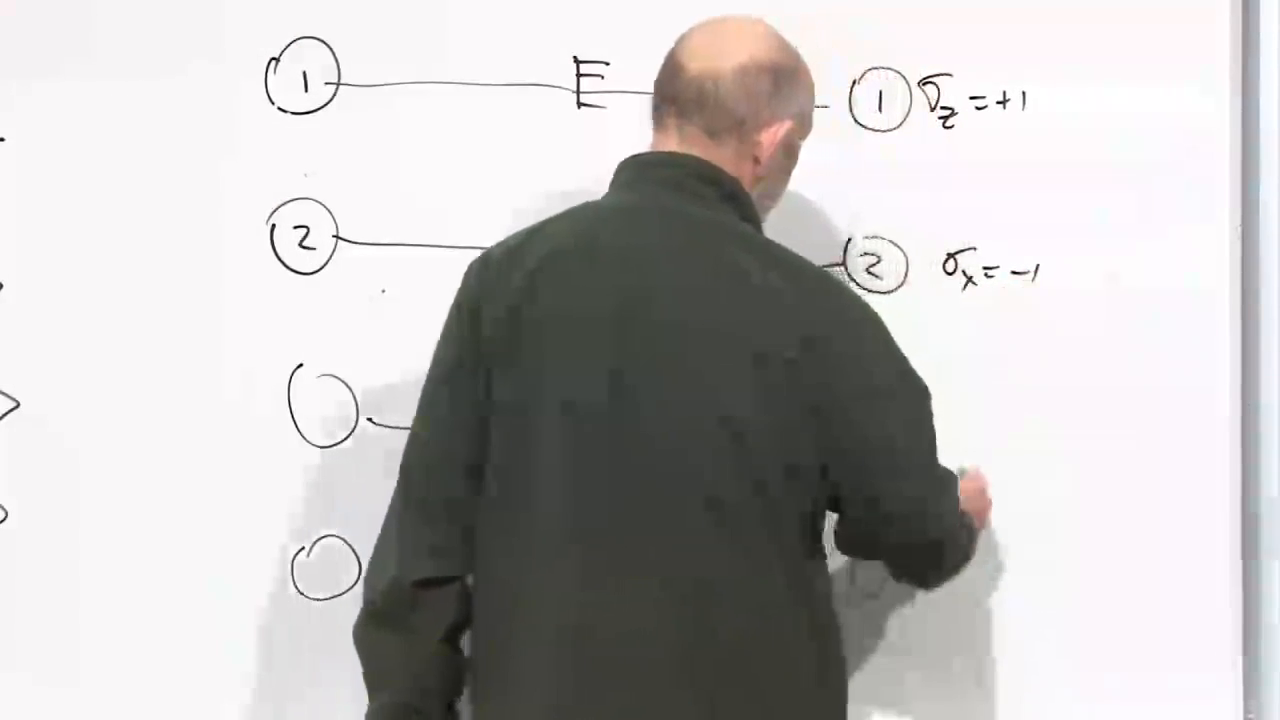
\includegraphics[width=0.88\textwidth]{lecture_07_figure_06.png}
\caption{對 Bob 的基底標記求和，便得到 Alice 的密度矩陣。}
\lectureframe{01:02:33}
\end{figure}

約化密度矩陣是厄米、半正定且歸一化的：
\begin{equation}
\rho_A^\dagger=\rho_A,
\qquad
\bra{\chi}\rho_A\ket{\chi}\geq0,
\qquad
\operatorname{Tr}\rho_A=1.
\label{eq:l7-density-properties}
\end{equation}
它完整包含了 Alice 進行所有局域測量所需的資訊。若兩個整體態產生相同的 \(\rho_A\)，任何只涉及 Alice 的實驗都無法區分這兩個態。

\begin{classroomqa}
\audiencequestion{Alice 會把密度矩陣當成一個可觀測量來測量嗎？}
\lecturerresponse{無法在單次測量中這麼做。密度矩陣是計算所有局域測量機率的依據。若有許多以相同方式製備的系統，Alice 可以透過量子態層析重建密度矩陣：她測量足夠的一組可觀測量，再由其期望值推得矩陣。}
\end{classroomqa}

\begin{classroomqa}
\audiencequestion{為什麼要對 Bob 求和，而不是選取 Bob 的某個態？}
\lecturerresponse{因為 Alice 沒有從 Bob 那裡取得任何測量結果資訊。偏跡是對 Bob 的完備基底求和，藉此得到非條件的局域態。若改為選取 Bob 的某個測量結果，得到的會是條件態；這是不同的操作，而且必須知道該結果。}
\end{classroomqa}

對乘積態 \(\Psi(a,b)=\psi_A(a)\phi_B(b)\) 而言，
\begin{align}
(\rho_A)_{aa'}
&=\sum_b
\psi_A(a)\phi_B(b)
\psi_A^*(a')\phi_B^*(b) \\
&=\psi_A(a)\psi_A^*(a')
\sum_b|\phi_B(b)|^2 \\
&=\psi_A(a)\psi_A^*(a').
\end{align}
因此
\begin{equation}
\rho_A=\ket{\psi_A}\bra{\psi_A}.
\label{eq:l7-pure-projector}
\end{equation}
這是一個秩一投影算符。作用於 \(\ket{\psi_A}\) 時，得到
\begin{equation}
\rho_A\ket{\psi_A}
=\ket{\psi_A}\braket{\psi_A}{\psi_A}
=\ket{\psi_A},
\label{eq:l7-density-on-state}
\end{equation}
而對任何與 \(\ket{\psi_A}\) 正交的 \(\ket{\chi}\)，
\begin{equation}
\rho_A\ket{\chi}
=\ket{\psi_A}\braket{\psi_A}{\chi}
=0.
\label{eq:l7-density-on-orthogonal}
\end{equation}

\begin{figure}[htbp]
\centering
\includegraphics[width=0.88\textwidth]{lecture_07_figure_07.png}
\caption{乘積態的密度矩陣可作為投影算符：沿著 \(\ket{\psi_A}\) 的本徵值為 \(1\)，正交向量上的本徵值則為 \(0\)。}
\lectureframe{01:09:43}
\end{figure}

\section{密度矩陣的譜與糾纏}

\(\rho_A\) 的本徵值皆為非負，且總和為一。對於整體的純態：
\begin{itemize}
\item 若恰好只有一個非零本徵值，且該值等於 \(1\)，則此態是乘積態；
\item 若非零本徵值多於一個，則此態是糾纏態；
\item 若本徵值在所有可用的局域支撐空間上相等，則為最大糾纏態。
\end{itemize}
施密特分解最能清楚呈現這項陳述：
\begin{equation}
\begin{aligned}
\ket{\Psi}_{AB}
&=\sum_{r=1}^{R}\sqrt{\lambda_r}
\ket{r}_A\ket{r}_B,\\
\lambda_r&\geq0,
\qquad
\sum_r\lambda_r=1.
\end{aligned}
\label{eq:l7-schmidt}
\end{equation}
此時
\begin{equation}
\rho_A=\sum_{r=1}^{R}\lambda_r\ket{r}_A\bra{r}.
\label{eq:l7-schmidt-density}
\end{equation}
乘積態的施密特秩 \(R\) 為一；糾纏純態的施密特秩則大於一。

對單態而言，
\begin{equation}
\rho_A
=\operatorname{Tr}_B\ket{S}\bra{S}
=\frac12\ket{u}\bra{u}
+\frac12\ket{d}\bra{d}
=\frac12 I.
\label{eq:l7-singlet-reduced-density}
\end{equation}
其本徵值為
\begin{equation}
\operatorname{spec}(\rho_A)
=\left\{\frac12,\frac12\right\}.
\end{equation}
儘管整對系統處於純態，Alice 的局域態卻是最大混合態。

密度矩陣的譜也提示了一種定量度量。馮紐曼熵
\begin{equation}
S(\rho_A)
=-\operatorname{Tr}(\rho_A\log\rho_A)
=-\sum_r\lambda_r\log\lambda_r
\label{eq:l7-entanglement-entropy}
\end{equation}
在乘積純態時為零；當 \(d_A\leq d_B\) 時，最大糾纏態的熵則達到 \(\log d_A\)。熵的詳細應用可以留待稍後討論；光是密度矩陣的譜就已呈現核心差異。

\begin{classroomqa}
\audiencequestion{糾纏態的約化密度矩陣，每個本徵值都必須非零嗎？}
\lecturerresponse{不必。只要有多於一個非零本徵值就足夠。若 Alice 的空間維度很大，糾纏態可能只占據較低維度的施密特子空間，因此還有其他本徵值為零。最大糾纏表示在較小子系統的整個空間上本徵值相等，而不只是任意挑選的一部分本徵值相等。}
\end{classroomqa}

\begin{classroomqa}
\audiencequestion{約化密度矩陣是混合態，本身就能證明 Alice 與 Bob 彼此糾纏嗎？}
\lecturerresponse{只有在已知整體態為純態時才可以。混合的局域態也可能來自混合整體態中的一般古典混合。不過，對純雙體態而言，局域態為混合態，恰好等同於兩部分之間存在糾纏。}
\end{classroomqa}

\begin{classroomqa}
\audiencequestion{Alice 的可觀測量的所有矩，都能決定她的機率分布嗎？}
\lecturerresponse{對有限維系統而言，算符基底的期望值可以決定 \(\rho_A\)；而 \(\rho_A\) 可透過波恩定則決定每一種局域測量結果的分布。重建需要多個以相同方式製備的系統副本；單一事件無法揭示密度矩陣。}
\end{classroomqa}

\section{測量作為糾纏相互作用}

將 Alice 和 Bob 換成一個自旋與一個測量儀器。設儀器有一個待命態 \(\ket{0}_D\) 和一個觸發態 \(\ket{1}_D\)。若要記錄自旋是否向上，理想相互作用可表示為
\begin{align}
\ket{u}\ket{0}_D&\longrightarrow\ket{u}\ket{1}_D,\\
\ket{d}\ket{0}_D&\longrightarrow\ket{d}\ket{0}_D.
\label{eq:l7-measurement-basis-map}
\end{align}
探測器必須從已知的待命態開始；否則其最終態就無法提供明確的紀錄。

線性性決定了疊加態的演化：
\begin{equation}
\left(\alpha\ket{u}+\beta\ket{d}\right)\ket{0}_D
\longrightarrow
\alpha\ket{u}\ket{1}_D
+\beta\ket{d}\ket{0}_D.
\label{eq:l7-measurement-entanglement}
\end{equation}
只要兩個係數都不為零，末態就是糾纏態。儀器之所以取得資訊，正是因為指標態與自旋相關聯。

\begin{figure}[htbp]
\centering
\includegraphics[width=0.88\textwidth]{lecture_07_figure_08.png}
\caption{理想測量將自旋的不同可能狀態與不同指標態建立關聯，因而產生糾纏。}
\lectureframe{01:20:20}
\end{figure}

若只保留自旋、忽略探測器，其約化態為
\begin{equation}
\rho_{\mathrm{spin}}
=|\alpha|^2\ket{u}\bra{u}
+|\beta|^2\ket{d}\bra{d},
\label{eq:l7-postmeasurement-reduced-state}
\end{equation}
此處假設指標紀錄彼此正交。干涉項已從局域描述中消失，因為它們保存在自旋與儀器的關聯之中。

現在有兩種互補的描述。若讀取探測器的結果，並依據紀錄作條件化，自旋便被指定為相應的分支：觸發後為 \(\ket{u}\)，未觸發後為 \(\ket{d}\)。這就是坍縮描述。若將探測器與自旋視為一個封閉系統，式~\eqref{eq:l7-measurement-entanglement}描述的就是一般的么正演化，聯合態中並沒有任何分支被移除。

\begin{classroomqa}
\audiencequestion{測量是超越糾纏之外的某種事物嗎？}
\lecturerresponse{就系統--儀器的動力學而言，測量是建立可靠關聯的一種相互作用。選定一筆確定紀錄後所使用的，是坍縮的條件式描述。這種更新究竟是基本過程，還是相對於所選界線而言，屬於詮釋問題；兩種看法的操作性預測一致。}
\end{classroomqa}

\begin{classroomqa}
\audiencequestion{為什麼理想測量不會改變自旋本徵態？}
\lecturerresponse{這是此模型的可重複測量要求。若輸入態已是待測可觀測量的本徵態，儀器應記錄其值，而不改變該值。實際測量可能具有破壞性；若是如此，就必須用不同方式建立其相互作用模型。}
\end{classroomqa}

\section{觀察者的層級}

一旦將儀器納入量子系統，就沒有自然的理由在此止步。指標發出的光會與眼睛相互作用；眼睛傳出的訊號會與大腦建立關聯；一位觀察者也可能成為另一位觀察者觀察的對象。Schr\"odinger的貓與維格納的朋友，將同一種層層嵌套的結構戲劇化地呈現出來：
\begin{equation}
\begin{gathered}
\text{spin}
\longrightarrow
\text{apparatus}
\longrightarrow
\text{cat}\\
\longrightarrow
\text{Schr\"odinger}
\longrightarrow
\text{Wigner}.
\end{gathered}
\label{eq:l7-observer-chain}
\end{equation}
在任一選定界線之內，都可以用么正演化與逐漸增強的糾纏來描述這條鏈。界線之外，則使用以測量結果為條件的坍縮語言。

關鍵的一致性條件是，界線可以移動。如果貓記錄到自旋向上，Schr\"odinger之後就必須記錄一隻看到自旋向上的貓；而維格納也必須記錄Schr\"odinger記下了相同的經歷。量子力學並未指定一條唯一而明確的界線，規定客觀事件必須在哪裡宣告。貓、眼睛和大腦都由物理自由度構成；若要將其中任何一者排除於量子力學之外，就需要額外的定律。

對於由此產生的不安，費曼採取務實的態度。概念上的問題可能極為龐大，甚至難以確定該如何陳述它是否存在；與此同時，計算規則仍能預測它們所適用的每一項實驗。形式體系的目的不是強迫人們接受某種詮釋，而是精確指出不安的來源：即使我們完整知道整體，也可能無法以純態描述其中任何部分。

\begin{classroomqa}
\audiencequestion{如果我是那隻貓，我必須把界線畫在自己身上嗎？}
\lecturerresponse{對你能取得的確定紀錄，你可以採用坍縮描述。另一位將你納入更大孤立系統的觀察者，則可以採用糾纏態描述。要求不在於每個人都畫下相同的界線，而在於觀察者日後比較結果時，各種描述都能給出一致的紀錄。}
\end{classroomqa}

\begin{classroomqa}
\audiencequestion{客觀事件發生在哪裡：原子、貓、Schr\"odinger，還是維格納？}
\lecturerresponse{么正形式體系沒有把這些位置中的任何一處選為特定界線。或許「\emph{發生}」這類日常用語，已被用在無法精確界定的語境中。形式工具告訴我們關聯如何傳遞，以及每位觀察者能預測什麼；至於如何詮釋最終的界線，則是另一回事。}
\end{classroomqa}

\subsection{弱耦合與不完全讀出}

式~\eqref{eq:l7-measurement-basis-map}中的理想映射會產生完全可區分的紀錄。較弱的相互作用可能使儀器態只有部分可區分：
\begin{equation}
\alpha\ket{u}\ket{D_u}
+\beta\ket{d}\ket{D_d},
\qquad
0<|\braket{D_d}{D_u}|<1.
\label{eq:l7-weak-measurement}
\end{equation}
此時儀器只取得部分資訊，糾纏也不完全。這就是弱測量或非銳利測量的情況。

這種情況必須與後續讀出不良區分開來。探測器可能已與自旋完全建立關聯，但眼睛、纜線、放大器或大腦未能清楚傳遞紀錄。前一種情況是系統--探測器之間的相互作用較弱；後一種情況則是探測器已有良好紀錄，但後續資訊傳遞的效率不佳。探測器效率可能涉及其中任一階段，因此在判定原因前，必須先確認實際的物理耦合。

\begin{classroomqa}
\audiencequestion{如果視力不佳，讓你無法確定指針的讀值，這是否表示量子測量是弱測量？}
\lecturerresponse{不一定。自旋可能已與儀器強烈且完全地關聯，但從儀器到眼睛，或從眼睛到大腦的通道可能不佳。真正的弱測量，指的是初始的系統--儀器耦合本身只產生了部分可區分的記錄。}
\end{classroomqa}

\section{局域性與無訊號傳遞}

應為「\emph{超距作用}」這個說法賦予操作上的意義。在一般物理學中，遠處的作用會改變此處可觀測到的結果。假如太陽消失後，地球的運動立即改變，而不是等到光傳播所需的時間過後才改變，我們就能利用這種變化以超光速傳遞資訊。那才是真正的非定域訊號傳遞。

糾纏無法用來傳遞這種訊號。設Bob執行一個以Kraus算符\(K_\mu\)表示的局域量子操作，其中
\begin{equation}
\sum_\mu K_\mu^\dagger K_\mu=I_B.
\end{equation}
如果Alice不知道Bob得到的結果，最終的聯合態為
\begin{equation}
\rho'_{AB}
=\sum_\mu
(I_A\otimes K_\mu)\rho_{AB}
(I_A\otimes K_\mu^\dagger).
\end{equation}
對Bob取偏跡，可得
\begin{equation}
\rho'_A
=\operatorname{Tr}_B\rho'_{AB}
=\operatorname{Tr}_B\rho_{AB}
=\rho_A.
\label{eq:l7-no-signaling}
\end{equation}
因此，Bob選擇任何保跡的局域操作，都不會改變Alice局域測量的無條件機率。

條件態則有所不同。如果Bob測量後得到結果\(\mu\)，Alice可以指派下列狀態：
\begin{equation}
\rho_{A|\mu}
=\frac{
\operatorname{Tr}_B\!\left[
(I_A\otimes K_\mu)\rho_{AB}
(I_A\otimes K_\mu^\dagger)
\right]
}{p_\mu}.
\label{eq:l7-conditioned-state}
\end{equation}
但在Bob透過一般訊號傳來\(\mu\)之前，Alice無從得知哪一個\(\rho_{A|\mu}\)適用。在訊息抵達之前，她必須對所有結果取平均：
\begin{equation}
\sum_\mu p_\mu\rho_{A|\mu}=\rho_A.
\label{eq:l7-conditioned-average}
\end{equation}

\begin{classroomqa}
\audiencequestion{如果Bob先測量，Alice的密度矩陣何時會改變？}
\lecturerresponse{她的無條件密度矩陣不會改變。等Bob的測量結果傳到她那裡，她才可以用相應的條件密度矩陣取代原來的矩陣。這項更新反映的是新取得的資訊，在古典訊息抵達之前無法使用。}
\end{classroomqa}

\begin{classroomqa}
\audiencequestion{Bob的測量會在同一瞬間使Alice的態發生物理坍縮嗎？}
\lecturerresponse{不同詮釋對條件更新有不同描述，但都同意一項可檢驗的陳述：在Bob的資訊可供Alice取得之前，她局域測量的結果機率維持不變。不會因此產生任何可控的瞬時訊號。}
\end{classroomqa}

設想許多單態對分散在編號列中。Bob對其中一對測量\(z\)，對另一對測量\(x\)，再對另一對測量\(y\)，依此類推。對每一列而言，Alice局域測得的結果序列都維持無偏：
\begin{equation}
P_A(+|\mathbf a)=P_A(-|\mathbf a)=\frac12.
\label{eq:l7-alice-marginal}
\end{equation}
她的紀錄中沒有任何線索能揭示Bob選了哪些測量軸，或得到了哪些結果。

\begin{figure}[htbp]
\centering
\includegraphics[width=0.88\textwidth]{lecture_07_figure_09.png}
\caption{許多獨立製備的粒子對，讓我們可以將不同的測量軸分配給不同列；Alice的邊際統計始終不變。}
\lectureframe{01:49:00}
\end{figure}

受光速限制的電報抵達後，列出Bob在每一列採用的測量軸和所得結果，Alice便能整理自己的紀錄。對單態對沿相同軸測量，兩人的結果就會逐對相反。這則訊息揭示的是聯合統計中原已存在的關聯，不會追溯改變Alice先前的局域頻率分布。

\begin{classroomqa}
\audiencequestion{Alice能否從自己的資料中取得足夠多階的統計矩，進而推斷Bob的選擇？}
\lecturerresponse{不能。所有Alice局域的統計矩都由\(\rho_A\)決定，而方程式~\eqref{eq:l7-no-signaling}表明該矩陣保持不變。增加副本數量，只會讓她更準確地估計同一個局域密度矩陣；仍無法得知Bob採用的基底或得到的結果。}
\end{classroomqa}

\begin{classroomqa}
\audiencequestion{如果Bob對系綜中的每個成員都選擇不同的測量軸呢？}
\lecturerresponse{Alice看到的局域分布仍然相同。等Bob傳來逐列的設定和結果後，雙方就能比較每一對測量軸所對應的條件關聯。設定的影響出現在聯合統計中，不會出現在Alice的邊際統計中。}
\end{classroomqa}

\section{作為模擬遊戲的Bell問題}

把無訊號傳遞和Bell非定域性的差異視為經典模擬問題，會讓這個差異更加清楚。先考慮一個自旋：
\begin{equation}
\ket{\psi}=\alpha_u\ket{u}+\alpha_d\ket{d},
\qquad
|\alpha_u|^2+|\alpha_d|^2=1.
\end{equation}
經典程式可以儲存兩個複振幅，依照Schr\"odinger方程式使它們演化，並接受使用者選定的測量方向。收到測量指令時，程式會計算Born機率，利用偽隨機數產生器選出一個結果、顯示結果，並將儲存的狀態更新為相應的本徵態。重複這個過程，就能再現單一自旋的統計。

因此，隨機性本身並不是經典力學與量子力學的分界。經典電腦也能產生在操作上足夠隨機、可用於模擬的序列，即使底層的偽隨機演算法是確定性的。

對於處於乘積態的兩個自旋，兩台分開的電腦也足以完成模擬。Alice的電腦儲存並演化\(\ket{\psi_A}\)；Bob的電腦則儲存並演化\(\ket{\phi_B}\)。每台電腦只對自己的局域設定作出回應。由於聯合機率可因式分解，兩台電腦分開之後不需要通訊。

糾纏對讓問題變得不同。實驗前，可以先把兩台機器放在一起，載入彼此關聯的隱變數資料、同步時鐘，甚至給它們相同的隨機種子。然而分開之後，每個輸出都只能取決於本地的測量設定，以及事先提供的共享資訊。Bell定理指出，對於自由選定的測量設定，這類局域隱變數方案都無法再現所有量子關聯。

\begin{figure}[htbp]
\centering
\includegraphics[width=0.88\textwidth]{lecture_07_figure_10.png}
\caption{分開的電腦模型：局域程式可以共享製備資料，但分開後不能交換測量設定。}
\lectureframe{02:00:00}
\end{figure}

如果兩台電腦之間仍有連線，可以交換設定和結果，這種模擬就能再現那些關聯。但此時它們已不再構成真正分開的局域模型，而是共同運作為一台連線的電腦。問題不在於抽象的經典計算本身。單一的全域經典電腦可以儲存完整的聯合波函數，藉此模擬有限的量子系統；不過，所需記憶體通常會隨子系統數量呈指數增長。Bell定理所指出的障礙，針對的是由各自獨立運作的局域電腦所構成的模型。

\begin{classroomqa}
\audiencequestion{為什麼兩台電腦不能直接使用相同的隨機數序列？}
\lecturerresponse{局域隱變數模型本來就允許共享隨機性。共享的隨機性可以預先決定彼此關聯的答案，但每一側的答案都必須適用於該側日後可能選擇的所有測量設定。Bell不等式表述了所有這類預先安排的局域策略必須遵守的限制，而量子關聯違反了這些限制。}
\end{classroomqa}

\begin{classroomqa}
\audiencequestion{隨機數必須取決於測量方向嗎？}
\lecturerresponse{局域輸出可以取決於本地方向和共享的隱變數資料，但不能取決於分開後才選定的遠端方向。若允許輸出取決於兩邊的設定，就需要通訊、逆因果性，或放棄通常的測量獨立性假設。Bell定理明確列出這些假設，不把它們藏在「\emph{隨機}」一詞之中。}
\end{classroomqa}

\begin{classroomqa}
\audiencequestion{兩台分開的量子電腦能否做到經典程式做不到的事？}
\lecturerresponse{如果它們共享糾纏的量子自由度，就能做到。在這種情況下，電腦並非用局域的經典記錄來模擬糾纏，而是實際擁有糾纏。它們的局域測量結果仍無法傳遞可控的超光速訊息。}
\end{classroomqa}

\begin{classroomqa}
\audiencequestion{一台普通的經典電腦能模擬整個粒子對嗎？}
\lecturerresponse{可以。它能在同一處儲存四個聯合振幅，並計算所有測量機率。粒子數增加時，直接模擬會變得昂貴，因為希爾伯特空間的維度會呈指數增長；但只要所有資訊都能在一台電腦中全域存取，就不會有Bell矛盾。}
\end{classroomqa}

\begin{classroomqa}
\audiencequestion{那麼，Bell定理是否證明了通常所說的超距作用？}
\lecturerresponse{它證明的是，符合Bell假設的局域隱變數解釋無法再現觀測到的關聯。它並未提供讓Alice或Bob超光速傳遞訊號的通道。Bell非定域性和操作上超光速傳遞訊息，是兩種不同的主張。}
\end{classroomqa}

\section{局域能得知什麼？}

局域可觀測量與聯合可觀測量不可混為一談。Bob可以測量\(\sigma_x\)，Alice可以測量\(\tau_x\)；之後比較兩人的紀錄，就能估計
\begin{equation}
\expect{\sigma_x\tau_x}.
\end{equation}
單獨一方的局域裝置都無法測量這個乘積。旋轉純量
\begin{equation}
\boldsymbol{\sigma}\cdot\boldsymbol{\tau}
=\sigma_x\tau_x+\sigma_y\tau_y+\sigma_z\tau_z
\end{equation}
若要測量，就必須將三項分別安排在不同子系綜中測量，或使用能分辨單態與三重態子空間的新型聯合裝置。使用原有的局域自旋測量儀，無法對同一對粒子測得三個彼此不相容的分量乘積。

\begin{classroomqa}
\audiencequestion{有沒有某些整體可觀測量，是Alice和Bob原有的裝置無法分別測量的？}
\lecturerresponse{有。像\(\sigma_x\tau_x\)這樣的單一乘積，可以各自進行局域\(x\)測量，再透過比較結果估計。\(\boldsymbol{\sigma}\cdot\boldsymbol{\tau}\)卻無法由同一對粒子的同時\(x,y,z\)讀值拼湊出來。要測量它，需要真正的聯合單態--三重態測量，或是將互不相容的各項分別安排在不同系綜中測量。}
\end{classroomqa}

Bob無法從單次事件判斷是否有糾纏。不過，若有許多以相同方式製備的副本，他就能重建自己的約化密度矩陣。對量子位元而言，
\begin{equation}
\rho_B
=\frac12\left(
I+\mathbf r\cdot\boldsymbol{\sigma}
\right),
\label{eq:l7-bloch-density}
\end{equation}
沿著數個軸測量，便能確定Bloch向量\(\mathbf r\)。若\(|\mathbf r|=1\)，Bob的局域態就是純態；若\(|\mathbf r|<1\)，則是混合態。若已知每次試驗中的全域製備都是同一個純態，這種局域混合性就能證明Bob與其子系統以外的某個系統存在糾纏。

對於兩個純自旋組成的乘積態，Bob可以尋找極化方向\(\mathbf n=\mathbf r/|\mathbf r|\)。沿著該方向反覆測量，會得到同一個確定結果。對單態而言，\(\mathbf r=0\)，因此沿任何軸測量，局域結果都仍是隨機的。無論如何尋找，都找不到極化方向。

\begin{classroomqa}
\audiencequestion{Bob能不和Alice交談，就發現糾纏嗎？}
\lecturerresponse{從一個系綜中，他可以發現自己的約化態是混合態。如果他還知道每一對粒子都是以相同的全域純態製備，就能推斷兩個子系統之間存在糾纏。若沒有純態這項假設，他的混合態也可能來自經典的製備混合；光憑局域資料，無法判定是哪一種情況。}
\end{classroomqa}

\begin{classroomqa}
\audiencequestion{為什麼需要許多以相同方式製備的系統？}
\lecturerresponse{每次自旋測量只會得到一個結果，而且通常會擾動該副本。因此，量子態層析會把彼此不相容的測量分配到一群以相同程序製備的系統上。密度矩陣及其譜是從重複試驗推斷出的統計性質，不是單一粒子所揭示的標籤。}
\end{classroomqa}

至此，整套論述回到了起點。糾纏不是含糊地共享某種狀態，而是純聯合態無法因式分解；這一點在局域上表現為約化密度矩陣不是投影算符，在聯合測量中則表現為分開的經典帳目無法再現的關聯。整體狀態可以完全確知，各個部分卻仍是混合態。正因如此，測量才成為可能，無訊號傳遞得以維持，也形成了Bell定理將要檢驗的結構。
